\section*{Chapitre 3}
\section{Conception Préliminaire}
\indent Cette étape nous permet, à partir des différents éléments de l'analyse, de mettre en forme les fonctions et procédures afin d'en expliciter les nouveaux fonctionnements.

\subsection{Cas d'utilisation}
\begin{figure}[h]
\centering
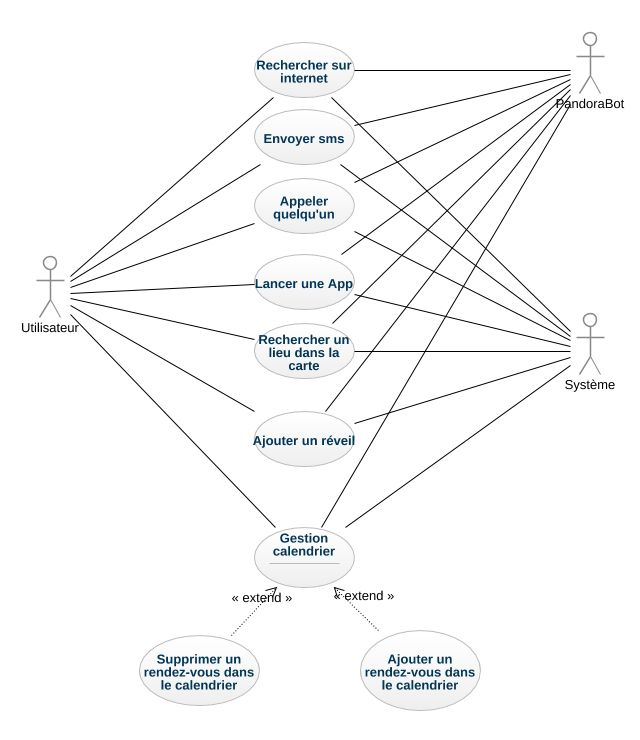
\includegraphics[scale=0.5]{./diagrammes/UsecaseDiagram.jpeg}
\caption{Cas d'utilisation.\label{fig2}}
\end{figure}

\subsection{Diagrammes de Sequence}
\begin{figure}[h]
\centering
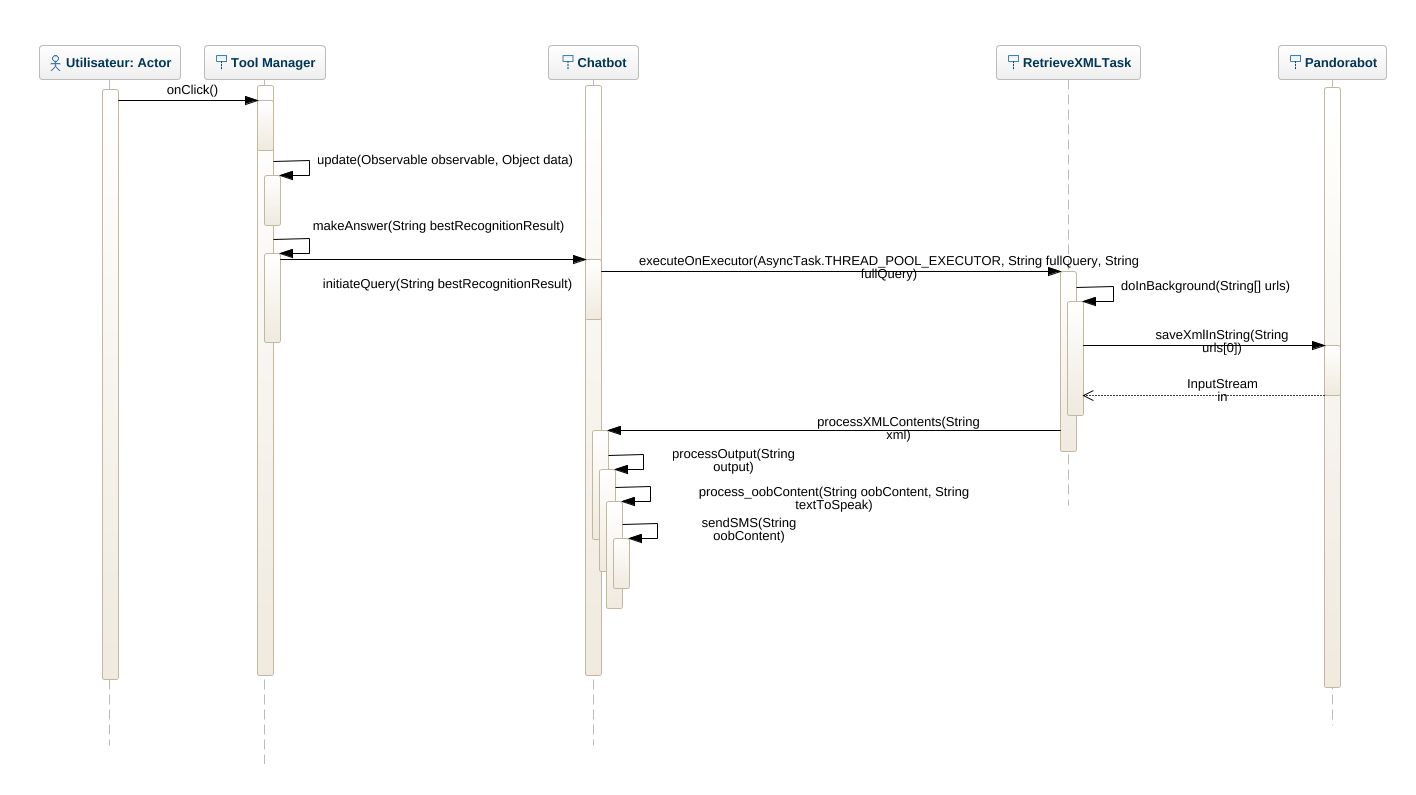
\includegraphics[scale=0.5]{./diagrammes/Sequence_diagramme_envoyer_un_sms.jpeg}
\caption{Diagramme de Sequence pour envoyer un sms.\label{fig3}}
\end{figure}
\indent C'est un diagramme de sequence pour envoyer un sms. Les parties à la boite noire est la partie du code qui a été complété dans les dernières versions. Nous vous donnons ce diagramme comme un model de diagramme de sequence. Pour autres fonctions ou procédures, nous travaillons en même mode.
\newpage


\subsection{Signatures Partie Chatbot}
procédure setAppointement (E/S Gcal : GestionCalendar, E oobContent : String, operationType : String)\\
\indent fonction setBeginTimeAndGetTitle (E oobContent : String, beginTime : Calendar, operationType : String) : String\\
\indent procédure googleQuery (E/S googleSearchText : String)\\
\indent procédure lauchApp (E app : String)\\
\indent procédure lauchUrl (E/S url : String)\\
\indent procédure lauchGoogleMap (E/S address : String)\\
\indent procédure sendSMS (E oobContent : String)\\
\indent procédure makePhoneCall (E oobContent : String)\\
\indent procédure addAnAlarm(E oobContent : String)\\
\indent procédure deleteAnAlarm (E oobContent : String)\\

\subsection{Signatures Partie ToolManager}
procédure setNextEvent()\\
\indent fonction getNextEvent() : String\\
\newpage

